\documentclass[]{book}
\usepackage{lmodern}
\usepackage{amssymb,amsmath}
\usepackage{ifxetex,ifluatex}
\usepackage{fixltx2e} % provides \textsubscript
\ifnum 0\ifxetex 1\fi\ifluatex 1\fi=0 % if pdftex
  \usepackage[T1]{fontenc}
  \usepackage[utf8]{inputenc}
\else % if luatex or xelatex
  \ifxetex
    \usepackage{mathspec}
  \else
    \usepackage{fontspec}
  \fi
  \defaultfontfeatures{Ligatures=TeX,Scale=MatchLowercase}
\fi
% use upquote if available, for straight quotes in verbatim environments
\IfFileExists{upquote.sty}{\usepackage{upquote}}{}
% use microtype if available
\IfFileExists{microtype.sty}{%
\usepackage{microtype}
\UseMicrotypeSet[protrusion]{basicmath} % disable protrusion for tt fonts
}{}
\usepackage[margin=1in]{geometry}
\usepackage{hyperref}
\hypersetup{unicode=true,
            pdftitle={A BAE Book Example},
            pdfauthor={BAE Faculty},
            pdfborder={0 0 0},
            breaklinks=true}
\urlstyle{same}  % don't use monospace font for urls
\usepackage{natbib}
\bibliographystyle{apalike}
\usepackage{color}
\usepackage{fancyvrb}
\newcommand{\VerbBar}{|}
\newcommand{\VERB}{\Verb[commandchars=\\\{\}]}
\DefineVerbatimEnvironment{Highlighting}{Verbatim}{commandchars=\\\{\}}
% Add ',fontsize=\small' for more characters per line
\usepackage{framed}
\definecolor{shadecolor}{RGB}{248,248,248}
\newenvironment{Shaded}{\begin{snugshade}}{\end{snugshade}}
\newcommand{\KeywordTok}[1]{\textcolor[rgb]{0.13,0.29,0.53}{\textbf{#1}}}
\newcommand{\DataTypeTok}[1]{\textcolor[rgb]{0.13,0.29,0.53}{#1}}
\newcommand{\DecValTok}[1]{\textcolor[rgb]{0.00,0.00,0.81}{#1}}
\newcommand{\BaseNTok}[1]{\textcolor[rgb]{0.00,0.00,0.81}{#1}}
\newcommand{\FloatTok}[1]{\textcolor[rgb]{0.00,0.00,0.81}{#1}}
\newcommand{\ConstantTok}[1]{\textcolor[rgb]{0.00,0.00,0.00}{#1}}
\newcommand{\CharTok}[1]{\textcolor[rgb]{0.31,0.60,0.02}{#1}}
\newcommand{\SpecialCharTok}[1]{\textcolor[rgb]{0.00,0.00,0.00}{#1}}
\newcommand{\StringTok}[1]{\textcolor[rgb]{0.31,0.60,0.02}{#1}}
\newcommand{\VerbatimStringTok}[1]{\textcolor[rgb]{0.31,0.60,0.02}{#1}}
\newcommand{\SpecialStringTok}[1]{\textcolor[rgb]{0.31,0.60,0.02}{#1}}
\newcommand{\ImportTok}[1]{#1}
\newcommand{\CommentTok}[1]{\textcolor[rgb]{0.56,0.35,0.01}{\textit{#1}}}
\newcommand{\DocumentationTok}[1]{\textcolor[rgb]{0.56,0.35,0.01}{\textbf{\textit{#1}}}}
\newcommand{\AnnotationTok}[1]{\textcolor[rgb]{0.56,0.35,0.01}{\textbf{\textit{#1}}}}
\newcommand{\CommentVarTok}[1]{\textcolor[rgb]{0.56,0.35,0.01}{\textbf{\textit{#1}}}}
\newcommand{\OtherTok}[1]{\textcolor[rgb]{0.56,0.35,0.01}{#1}}
\newcommand{\FunctionTok}[1]{\textcolor[rgb]{0.00,0.00,0.00}{#1}}
\newcommand{\VariableTok}[1]{\textcolor[rgb]{0.00,0.00,0.00}{#1}}
\newcommand{\ControlFlowTok}[1]{\textcolor[rgb]{0.13,0.29,0.53}{\textbf{#1}}}
\newcommand{\OperatorTok}[1]{\textcolor[rgb]{0.81,0.36,0.00}{\textbf{#1}}}
\newcommand{\BuiltInTok}[1]{#1}
\newcommand{\ExtensionTok}[1]{#1}
\newcommand{\PreprocessorTok}[1]{\textcolor[rgb]{0.56,0.35,0.01}{\textit{#1}}}
\newcommand{\AttributeTok}[1]{\textcolor[rgb]{0.77,0.63,0.00}{#1}}
\newcommand{\RegionMarkerTok}[1]{#1}
\newcommand{\InformationTok}[1]{\textcolor[rgb]{0.56,0.35,0.01}{\textbf{\textit{#1}}}}
\newcommand{\WarningTok}[1]{\textcolor[rgb]{0.56,0.35,0.01}{\textbf{\textit{#1}}}}
\newcommand{\AlertTok}[1]{\textcolor[rgb]{0.94,0.16,0.16}{#1}}
\newcommand{\ErrorTok}[1]{\textcolor[rgb]{0.64,0.00,0.00}{\textbf{#1}}}
\newcommand{\NormalTok}[1]{#1}
\usepackage{longtable,booktabs}
\usepackage{graphicx,grffile}
\makeatletter
\def\maxwidth{\ifdim\Gin@nat@width>\linewidth\linewidth\else\Gin@nat@width\fi}
\def\maxheight{\ifdim\Gin@nat@height>\textheight\textheight\else\Gin@nat@height\fi}
\makeatother
% Scale images if necessary, so that they will not overflow the page
% margins by default, and it is still possible to overwrite the defaults
% using explicit options in \includegraphics[width, height, ...]{}
\setkeys{Gin}{width=\maxwidth,height=\maxheight,keepaspectratio}
\IfFileExists{parskip.sty}{%
\usepackage{parskip}
}{% else
\setlength{\parindent}{0pt}
\setlength{\parskip}{6pt plus 2pt minus 1pt}
}
\setlength{\emergencystretch}{3em}  % prevent overfull lines
\providecommand{\tightlist}{%
  \setlength{\itemsep}{0pt}\setlength{\parskip}{0pt}}
\setcounter{secnumdepth}{5}
% Redefines (sub)paragraphs to behave more like sections
\ifx\paragraph\undefined\else
\let\oldparagraph\paragraph
\renewcommand{\paragraph}[1]{\oldparagraph{#1}\mbox{}}
\fi
\ifx\subparagraph\undefined\else
\let\oldsubparagraph\subparagraph
\renewcommand{\subparagraph}[1]{\oldsubparagraph{#1}\mbox{}}
\fi

%%% Use protect on footnotes to avoid problems with footnotes in titles
\let\rmarkdownfootnote\footnote%
\def\footnote{\protect\rmarkdownfootnote}

%%% Change title format to be more compact
\usepackage{titling}

% Create subtitle command for use in maketitle
\newcommand{\subtitle}[1]{
  \posttitle{
    \begin{center}\large#1\end{center}
    }
}

\setlength{\droptitle}{-2em}

  \title{A BAE Book Example}
    \pretitle{\vspace{\droptitle}\centering\huge}
  \posttitle{\par}
    \author{BAE Faculty}
    \preauthor{\centering\large\emph}
  \postauthor{\par}
      \predate{\centering\large\emph}
  \postdate{\par}
    \date{2018-12-18}

\usepackage{booktabs}
\usepackage{amsthm}
\makeatletter
\def\thm@space@setup{%
  \thm@preskip=8pt plus 2pt minus 4pt
  \thm@postskip=\thm@preskip
}
\makeatother
\usepackage{booktabs}
\usepackage{longtable}
\usepackage{array}
\usepackage{multirow}
\usepackage[table]{xcolor}
\usepackage{wrapfig}
\usepackage{float}
\usepackage{colortbl}
\usepackage{pdflscape}
\usepackage{tabu}
\usepackage{threeparttable}
\usepackage{threeparttablex}
\usepackage[normalem]{ulem}
\usepackage{makecell}

\usepackage{amsthm}
\newtheorem{theorem}{Theorem}[chapter]
\newtheorem{lemma}{Lemma}[chapter]
\theoremstyle{definition}
\newtheorem{definition}{Definition}[chapter]
\newtheorem{corollary}{Corollary}[chapter]
\newtheorem{proposition}{Proposition}[chapter]
\theoremstyle{definition}
\newtheorem{example}{Example}[chapter]
\theoremstyle{definition}
\newtheorem{exercise}{Exercise}[chapter]
\theoremstyle{remark}
\newtheorem*{remark}{Remark}
\newtheorem*{solution}{Solution}
\begin{document}
\maketitle

{
\setcounter{tocdepth}{1}
\tableofcontents
}
\chapter{Introduction}\label{introduction}

This is a \emph{sample} book written in \textbf{Markdown}. This is a
great package written by
\href{https://bookdown.org/yihui/bookdown/}{Yihui Xie}. I am using his
template, and added some additional info I thought was useful along the
way! This is really a very succint tutorial, so take it as an
introduction to your discovery of Reproducible research!!

The \textbf{bookdown} package can be installed from CRAN or Github:

\begin{Shaded}
\begin{Highlighting}[]
\KeywordTok{install.packages}\NormalTok{(}\StringTok{"bookdown"}\NormalTok{)}
\CommentTok{# or the development version}
\CommentTok{# devtools::install_github("rstudio/bookdown")}
\end{Highlighting}
\end{Shaded}

Remember each Rmd file contains one and only one chapter, and a chapter
is defined by the first-level heading \texttt{\#}.

To compile this example to PDF, you need XeLaTeX. You are recommended to
install TinyTeX (which includes XeLaTeX):
\url{https://yihui.name/tinytex/}.

\chapter{Introduction: Text features}\label{intro}

The markdown syntax is very simple and this is one of the reasons why it
is so attractive. You can find all the syntax with
\href{https://www.rstudio.com/wp-content/uploads/2015/03/rmarkdown-reference.pdf}{this
R Markdown reference document}, but I thought I would go through them as
I have learned several tricks I could not easily find in the document.

\section{Paragraph Breaks and Forced Line
Breaks}\label{paragraph-breaks-and-forced-line-breaks}

To insert a break between paragraphs, include a single completely blank
line.

To force a line break, put \emph{two} blank spaces at the end of a line.

\begin{verbatim}
To insert a break between paragraphs, include a single completely blank line.

To force a line break, put _two_ blank spaces at the end of a line.
\end{verbatim}

\section{Headers}\label{headers}

The character \texttt{\#} at the beginning of a line means that the rest
of the line is interpreted as a section header. The number of
\texttt{\#}s at the beginning of the line indicates the level of the
section (1,2,3, etc.). For instance,
\texttt{Components\ of\ R\ Markdown} above is preceded by a single
\texttt{\#}, because it is of level 1 but \texttt{Headers} at the start
of this paragraph is preceded by \texttt{\#\#\#} because it is of level
3. Up to six levels are understood by Markdown. Do not interrupt these
headers by line-breaks. Make sure that in your .Rmd file, you leave a
blank line before a header, otherwise, \texttt{pandoc} will not render
it as a header.

\section{Italics and bold}\label{italics-and-bold}

\begin{verbatim}
*italics* and _italics_
\end{verbatim}

renders \emph{italics} and \emph{italics}

\begin{verbatim}
**bold** and __bold__
\end{verbatim}

renders \textbf{bold} and \textbf{bold}

\section{Supbscripts and
superscripts}\label{supbscripts-and-superscripts}

To write sub- and superscripts, like in
NO\textsubscript{3}\textsuperscript{-} or
PO\textsubscript{4}\textsuperscript{3-} write as

\begin{verbatim}
NO~3~^-^ or PO~4~^3-^
\end{verbatim}

PO\textsubscript{4}\textsuperscript{3-} does not look as neat as
\(PO_4^{3-}\)

\begin{verbatim}
PO~4~^3-^ does not look as neat as $PO_4^{3-}$
\end{verbatim}

but looks more seamless in a normal text because the former does not
appear as an \protect\hyperlink{inline-equations}{equation} while the
other does.

\section{Lists}\label{lists}

\begin{verbatim}
* unordered list
* item 2
    + sub-item 1                #4 <spaces> before +
    + sub-item 2                #4 <spaces> before +
\end{verbatim}

\begin{itemize}
\tightlist
\item
  unordered list
\item
  item 2

  \begin{itemize}
  \tightlist
  \item
    sub-item 1
  \item
    sub-item 2
  \end{itemize}
\end{itemize}

\begin{verbatim}
1. ordered list
2. item 2
    + sub-item 1                #4 <spaces> before +
    + sub-item 2                #4 <spaces> before +
\end{verbatim}

\begin{enumerate}
\def\labelenumi{\arabic{enumi}.}
\tightlist
\item
  ordered list
\item
  item 2

  \begin{itemize}
  \tightlist
  \item
    sub-item 1
  \item
    sub-item 2
  \end{itemize}
\end{enumerate}

In the ordered list, there is a subtlety unrevealed in the Rmardown
documentation, which is that the numbering \emph{always} increases, and
that \emph{only} the number value of the first item matters. So, one
cannot have a list in a decreasing order (which is too bad because when
one makes a list of his/her publications, it is nice to have a
decreasing order\ldots{}), and the only number that matters is the first
one. So this code

\begin{verbatim}
5. ordered list
7. item 2
2. item 2
                                # blank line for list to take into effect
    b. sub-item 1               #4 <spaces> before b
    a. sub-item 2  
\end{verbatim}

 renders this:

\begin{enumerate}
\def\labelenumi{\arabic{enumi}.}
\setcounter{enumi}{4}
\item
  ordered list
\item
  item 2
\item
  item 2

  \begin{enumerate}
  \def\labelenumii{\alph{enumii}.}
  \setcounter{enumii}{1}
  \tightlist
  \item
    sub-item 1\\
  \item
    sub-item 2
  \end{enumerate}
\end{enumerate}

\section{Quotations}\label{quotations}

\begin{quote}
R Markdown is, in particular, both ``free as in beer'' (you will never
pay a dollar for software to use it) and ``free as in speech'' (the
specification is completely open to all to inspect).
\end{quote}

Is a quotation from
\href{http://www.stat.cmu.edu/~cshalizi/rmarkdown/}{Dr Shalizi} which
code starts with a \texttt{\textgreater{}}

\begin{verbatim}
> R Markdown is, in particular, both "free as in beer" etc.
\end{verbatim}

\section{Computer type}\label{computer-type}

This is to differentiate regular text from \texttt{code\ text} so that
both can be easily differentiated: \texttt{R} vs R.

\begin{verbatim}
This is to differentiate regular text from `code text` so that both can be easily differentiated: `R` vs R.
\end{verbatim}

An entire paragraph of code which is rendered as a ``code box'' in html
(but not in pdf) starts with three ``back-ticks'', and end the same

\section{Symbols and Special
characters}\label{symbols-and-special-characters}

The principal keys, like the alphabet, are understood univocally across
platforms such as Windows, Mac OS, or Linux. However, there are special
characters such °, ² or µ that have different embedded codes across the
different platforms. For example, if you and your co-worker work on the
same document and one works using Windows and the other uses Mac, the
actual symbol in the code text may not show the same one from one to the
other plateform.

For example, if I write in an R markdown document ``10 m²'' and I have
added the ² symbol by typing on a PC ``Alt+0178'', as this corresponds
to the ascii code for ² in Windows, the same document open on a Mac will
render ``10 m?'', because it cannot interpret the embedded code for
²\ldots{}

Several consequences:

\begin{enumerate}
\def\labelenumi{\arabic{enumi}.}
\tightlist
\item
  \textbf{NEVER} use special characters in variable names in an
  \texttt{R} code,
\item
  in an R markdown document, use the HTML Number or HTML name in the
  text
\end{enumerate}

\href{https://www.ascii.cl/htmlcodes.htm}{HTML Number and Names} can be
found on this \href{https://www.ascii.cl/htmlcodes.htm}{ascii page} or
on this page for
\href{http://www.dionysia.org/html/entities/symbols.html}{greek letter
codes and some other symbols}

So to type T°C, m², µm, or pε you type like this

\begin{verbatim}
So to type T&deg;C, m&sup2;, &micro;m, or p&epsilon; you type like this
\end{verbatim}

Do not forget to add the ``;'' !!!

\chapter{Editing equations in R
Markdown}\label{editing-equations-in-r-markdown}

We do not write nearly as much math in our field than our colleagues in
statistics or math. But we do enough to have a bit of a tutorial. I have
borrowed this entire section from the
\href{http://www.stat.cmu.edu/~cshalizi/rmarkdown/\#math-in-r-markdown}{excellent
tutorial from Dr Shalizi} again. R Markdown gives you the syntax to
render complex mathematical formulas and derivations, and have them
displayed very nicely. Like code, the math can either be inline or set
off (displays).

\hypertarget{inline-equations}{\section{Inline
equations}\label{inline-equations}}

Inline math is marked off witha pair of dollar signs (\texttt{\$}), as
\(\pi r^2\) or \(e^{i\pi}\).

\begin{verbatim}
Inline math is marked off witha pair of dollar
signs (`$`), as $\pi r^2$ or $e^{i\pi}$.
\end{verbatim}

\section{Set off equations}\label{set-off-equations}

In the
\href{https://francoisbirgand.github.io/tutorial-RMarkdown_instructions.html}{R
markdown tutorial} I have other instructions about equations that are
really related to R markdown. I now prefer the way it is done in
\texttt{bookdown} much better, particularly for the referencing.

This simple LaTeX syntax

\begin{verbatim}
\begin{equation}
H_2O + H_2O \rightleftharpoons OH^- + H_3O^+
\label{eq:autoprotolysis}
\end{equation}
\end{verbatim}

yields

\begin{equation}
H_2O + H_2O \rightleftharpoons OH^- + H_3O^+
\label{eq:autoprotolysis}
\end{equation}

Notice that the number \eqref{eq:autoprotolysis} is automatically added as
you put in the text \texttt{\textbackslash{}@ref(eq:autoprotolysis)}.

Of course, it is possible to write a little more complicated equations.
The limit is LaTeX. I have not explored all what there is but here is an
example that was useful for me:

\begin{verbatim}
\begin{equation}
H_nA \rightleftharpoons H_{n-1}A^- + H^+ \hspace{0.6cm} K_{a1} = \frac{[H_{n-1}A^-][H^+]}{[H_nA]} \hspace{0.6cm} [H_{n-1}A^-] = [H_nA] \frac {K_{a1}}{[H^+]}\\
H_{n-1}A^- \rightleftharpoons H_{n-2}A^{2-} + H^+ \hspace{0.6cm} K_{a2} = \frac{[H_{n-2}A^{2-}][H^+]}{[H_{n-1}A]} \hspace{0.6cm} [H_{n-2}A^-] = [H_nA] \frac {K_{a1}K_{a2}}{[H^+]^2}\\
\\
\vdots \hspace{6cm} \vdots \hspace{6cm} \vdots\\
\\
HA^{(n-1)-} \rightleftharpoons A^{n-} + H^+ \hspace{0.6cm} K_{an} = \frac{[A^{n-}][H^+]}{[HA^{(n-1)-}]} \hspace{0.6cm} [A^{n-}] = [H_nA] \frac {K_{a1}K_{a2} \ldots  K_{an}}{[H^+]^n}\\

\label{eq:HnApoly}
\end{equation}
\end{verbatim}

yields

\begin{equation}
H_nA \rightleftharpoons H_{n-1}A^- + H^+ \hspace{0.6cm} K_{a1} = \frac{[H_{n-1}A^-][H^+]}{[H_nA]} \hspace{0.6cm} [H_{n-1}A^-] = [H_nA] \frac {K_{a1}}{[H^+]}\\
H_{n-1}A^- \rightleftharpoons H_{n-2}A^{2-} + H^+ \hspace{0.6cm} K_{a2} = \frac{[H_{n-2}A^{2-}][H^+]}{[H_{n-1}A]} \hspace{0.6cm} [H_{n-2}A^-] = [H_nA] \frac {K_{a1}K_{a2}}{[H^+]^2}\\
\\
\vdots \hspace{6cm} \vdots \hspace{6cm} \vdots\\
\\
HA^{(n-1)-} \rightleftharpoons A^{n-} + H^+ \hspace{0.6cm} K_{an} = \frac{[A^{n-}][H^+]}{[HA^{(n-1)-}]} \hspace{0.6cm} [A^{n-}] = [H_nA] \frac {K_{a1}K_{a2} \ldots  K_{an}}{[H^+]^n}\\
\label{eq:HnApoly}
\end{equation}

Again, you see that the numbering of the equation is automatic!!

\chapter{Code chunks}\label{code-chunks}

So this is one of the great beauties of the \texttt{R\ markdown}
platform: You insert text, equations, and code chunks! Code chunks are
used to run \texttt{R} code, \texttt{python} code, and others such as
\texttt{C} and \texttt{fortran} codes! In \texttt{bookdown}, one also
uses them to insert pictures, videos, and tables.

\section{Inserting pictures}\label{inserting-pictures}

This code:

yields:

\begin{figure}

{\centering 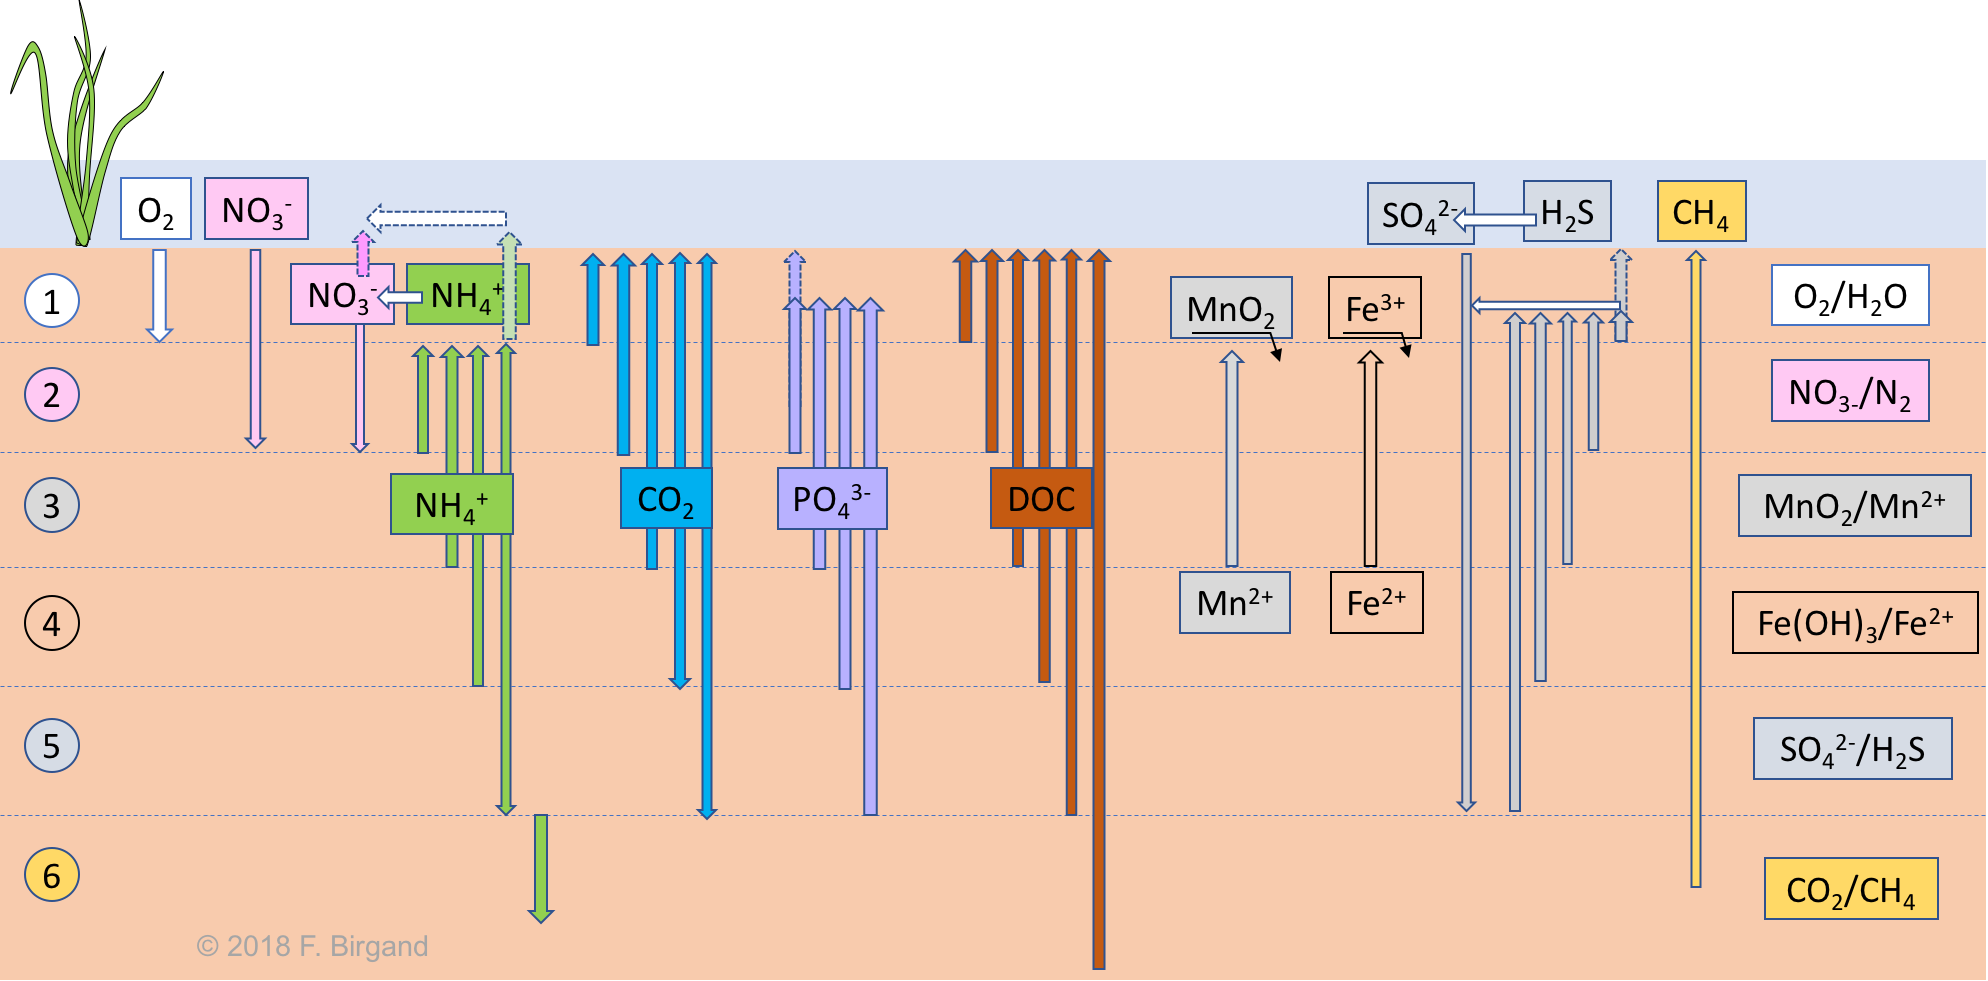
\includegraphics[width=1\linewidth]{pictures/diagenesis-diffusion-directions} 

}

\caption{Diffusion fluxes of electron acceptors and all other soil diagenesis processes of a theoretical layered wetland soil}\label{fig:diagenesis-diffusion-directions}
\end{figure}

So the first thing in the code is its name. It then becomes possible to
reference the figure using
\texttt{Figure\ \textbackslash{}@ref(fig:diagenesis-diffusion-directions)}
to say: look at the cool stuff in Figure
\ref{fig:diagenesis-diffusion-directions}. Then, there are other
settings for the code, which are detailed below. The figure caption is
announced with the \texttt{fig.cap=}.

\section{Inserting several pictures}\label{inserting-several-pictures}

It is also possible to insert several pictures lined up using this code:

which yields:

\begin{figure}

{\centering 
\includegraphics[width=0.4\linewidth]{pictures/brickwall} 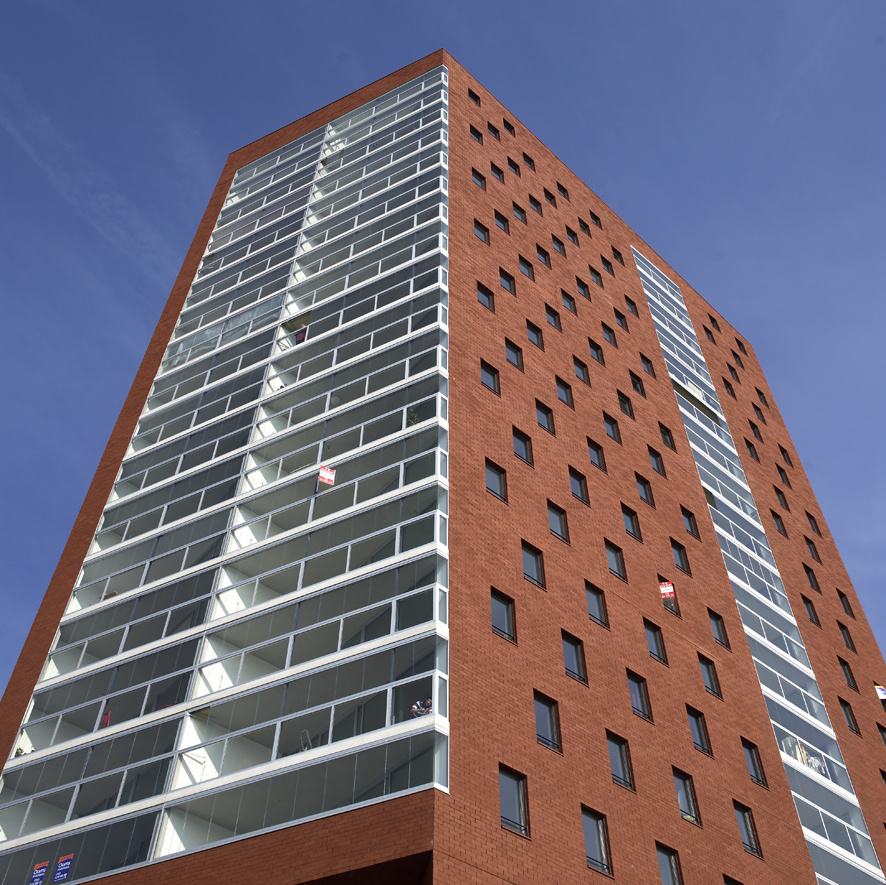
\includegraphics[width=0.4\linewidth]{pictures/brick-skyscraper} 

}

\caption{Small and large structures can be built from the addition of bricks, one at a time}\label{fig:brickwall}
\end{figure}

\section{Inserting videos}\label{inserting-videos}

Similarly, it is possible to insert videos from the web using this code:

which yields:

\label{fig:ATPaseRotation}ATP synthase in action. Obtained with permission
from HarvardX

\section{Inserting R code}\label{inserting-r-code}

And obviously, a nice thing about \texttt{R\ markdown} is to be able to
insert \texttt{R} code chunks like the one below to make some pretty
complicated figures (the one here is not that much, and is not
particularly well written\ldots{})

which yields:

\begin{figure}

{\centering 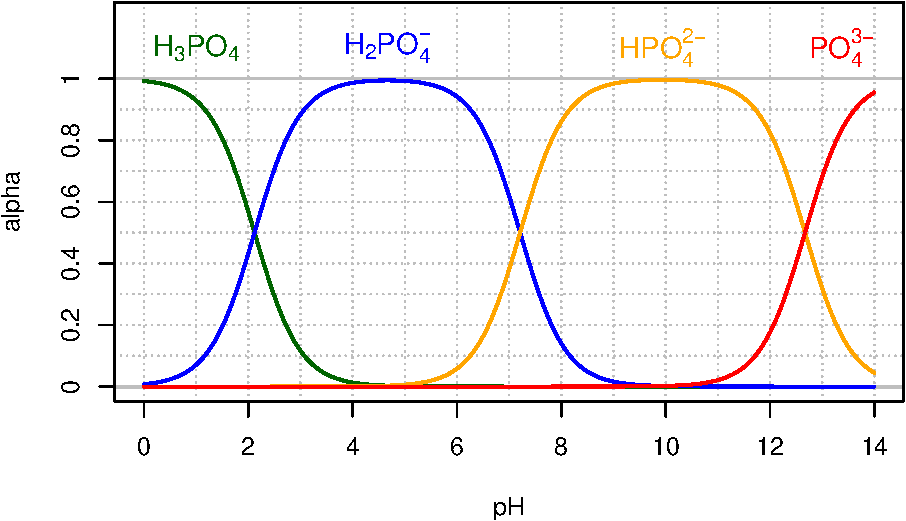
\includegraphics[width=0.85\linewidth]{bookdown-demo_files/figure-latex/molarfracPO4-1} 

}

\caption{Molar fraction for the conjugate acid forms of the triprotic phosphoric acid in dilute solutions at 25°C}\label{fig:molarfracPO4}
\end{figure}

\section{Inserting tables}\label{inserting-tables}

To me, this is where Rmarkdown is the weakest for now. Tables are not
that easy to handle\ldots{} Here is a Chunk code that works with
\texttt{pander}. I had to use this because otherwise, it would not
render the equations well, but it does not have a caption, which is what
I was trying to have anyway.

\begin{longtable}[]{@{}cc@{}}
\toprule
Equilibrium reactions & Log K\tabularnewline
\midrule
\endhead
H\textsuperscript{+} + OH\textsuperscript{-} ⇆ H\textsubscript{2}O &
-14.00\tabularnewline
H\textsuperscript{+} + e\textsuperscript{-} ⇆ H\textsubscript{2(g)} &
0.00\tabularnewline
H\textsuperscript{+} + e\textsuperscript{-} + ¼O\textsubscript{2(g)} ⇆
½H\textsubscript{2}O & 20.78\tabularnewline
\bottomrule
\end{longtable}

There is another package which I like in many ways, but it is still
imperfect: \texttt{KableExtra}. In the code below, it is possible to
insert picture with text.

The beauty is that I was able to get the caption here and this is very
useful. I suppose that for most applications, \texttt{KableExtra} is
still the best thing outthere. Again, to reference the table, use
\texttt{\textbackslash{}@ref(tab:ElecAllocTab)} to say that table
\ref{tab:ElecAllocTab} is very messy!!

\label{tab:ElecAllocTab}Examples of electron allocations on the C, N, S, and
P atoms generating different inorganic and organic molecules relevant to
environmental and ecological engineering

Nb of e\textsuperscript{-} stored on the atoms

C

N

S

P

0

carbon dioxide~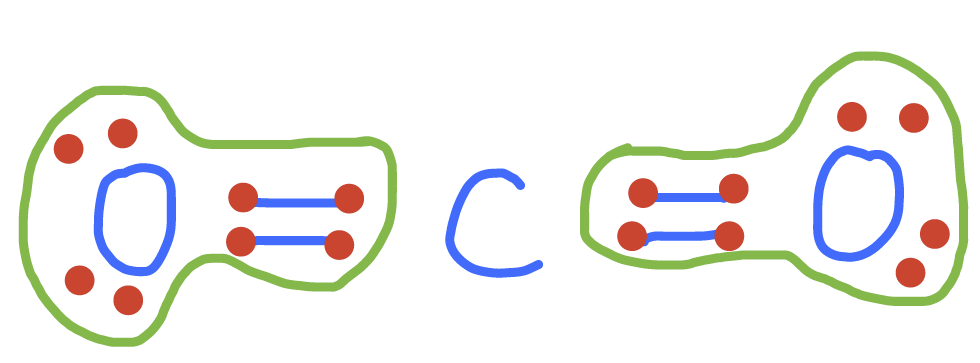
\includegraphics{pictures/ElecAlloc_CO2.png}

nitr\emph{\textbf{ate}}~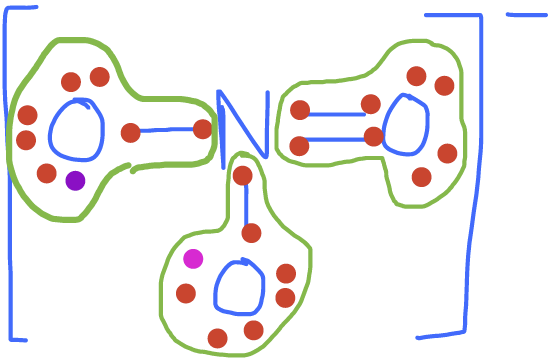
\includegraphics{pictures/ElecAlloc_NO3-.png}

sulf\emph{\textbf{ate}}~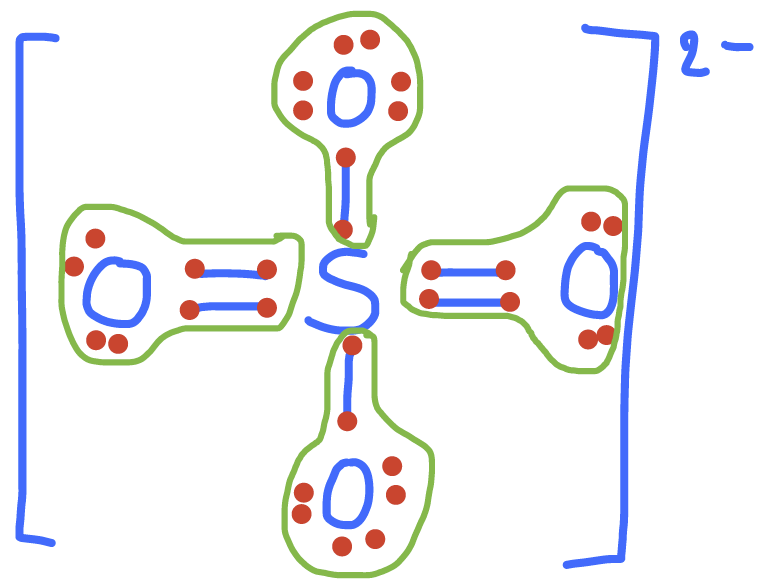
\includegraphics{pictures/ElecAlloc_SO42-.png}

phosph\emph{\textbf{ate}}~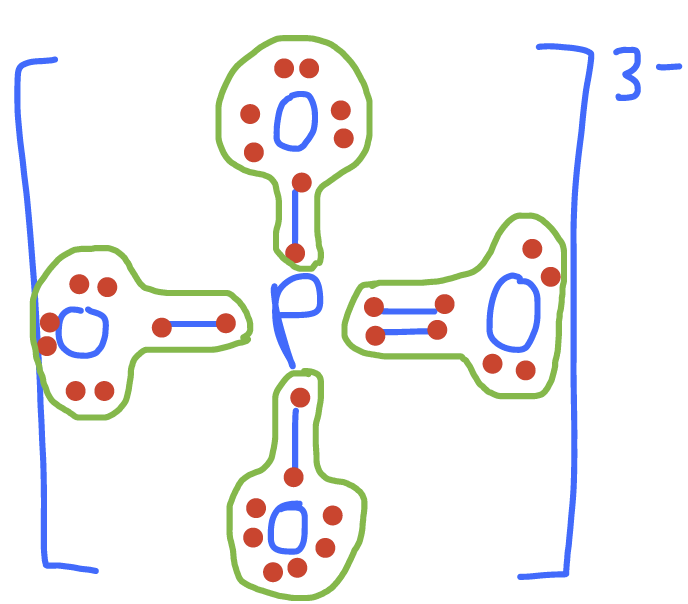
\includegraphics{pictures/ElecAlloc_PO43-.png}

1

C\#1 pyruvic acid~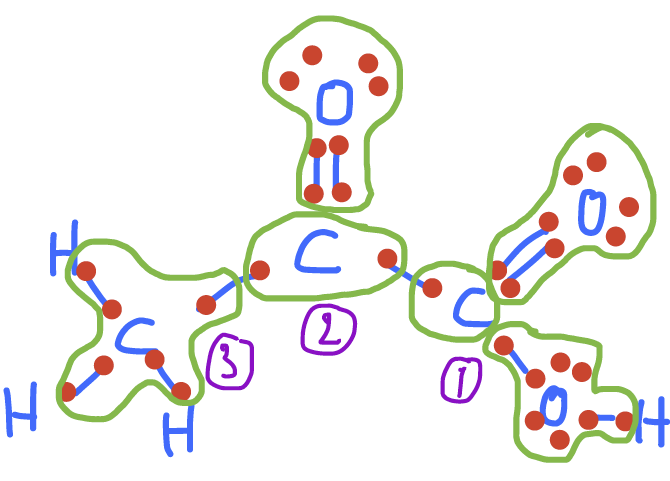
\includegraphics{pictures/ElecAlloc_pyruvic_acid.png}

2

C\#2 pyruvic acid~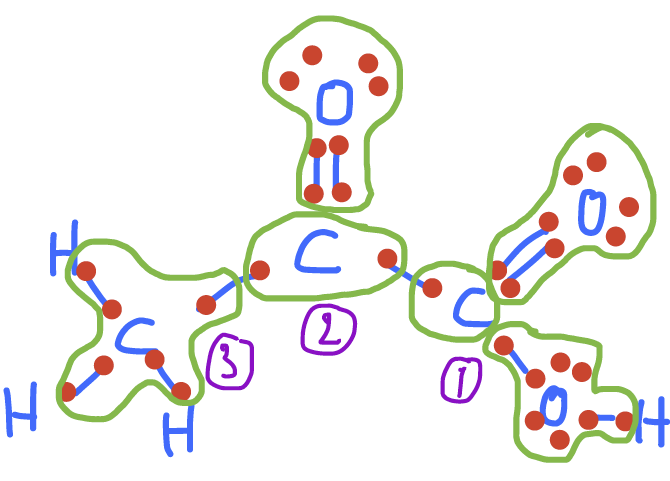
\includegraphics{pictures/ElecAlloc_pyruvic_acid.png}
carbon monoxide

\includegraphics[width=0.70000\textwidth]{pictures/ElecAlloc_CO.png}

nitr\emph{\textbf{ite}}~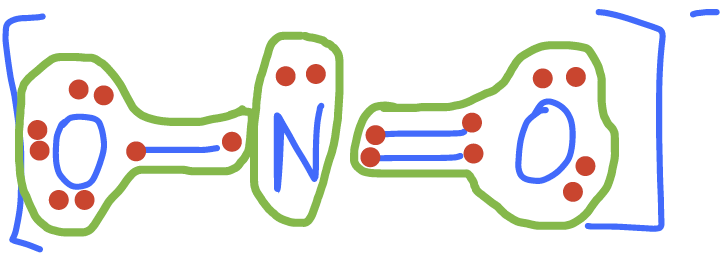
\includegraphics{pictures/ElecAlloc_NO2-.png}

sulf\emph{\textbf{ite}}~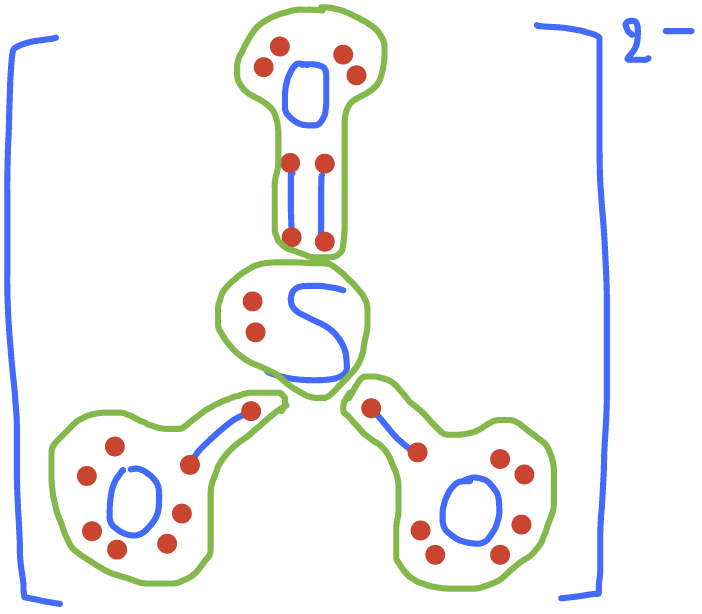
\includegraphics{pictures/ElecAlloc_SO32-.png}
sulfur dioxide ~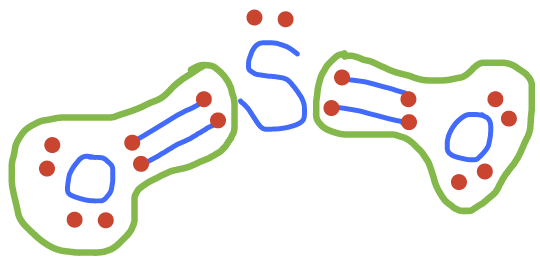
\includegraphics{pictures/ElecAlloc_SO2.png}

3

C\#1 of glucose~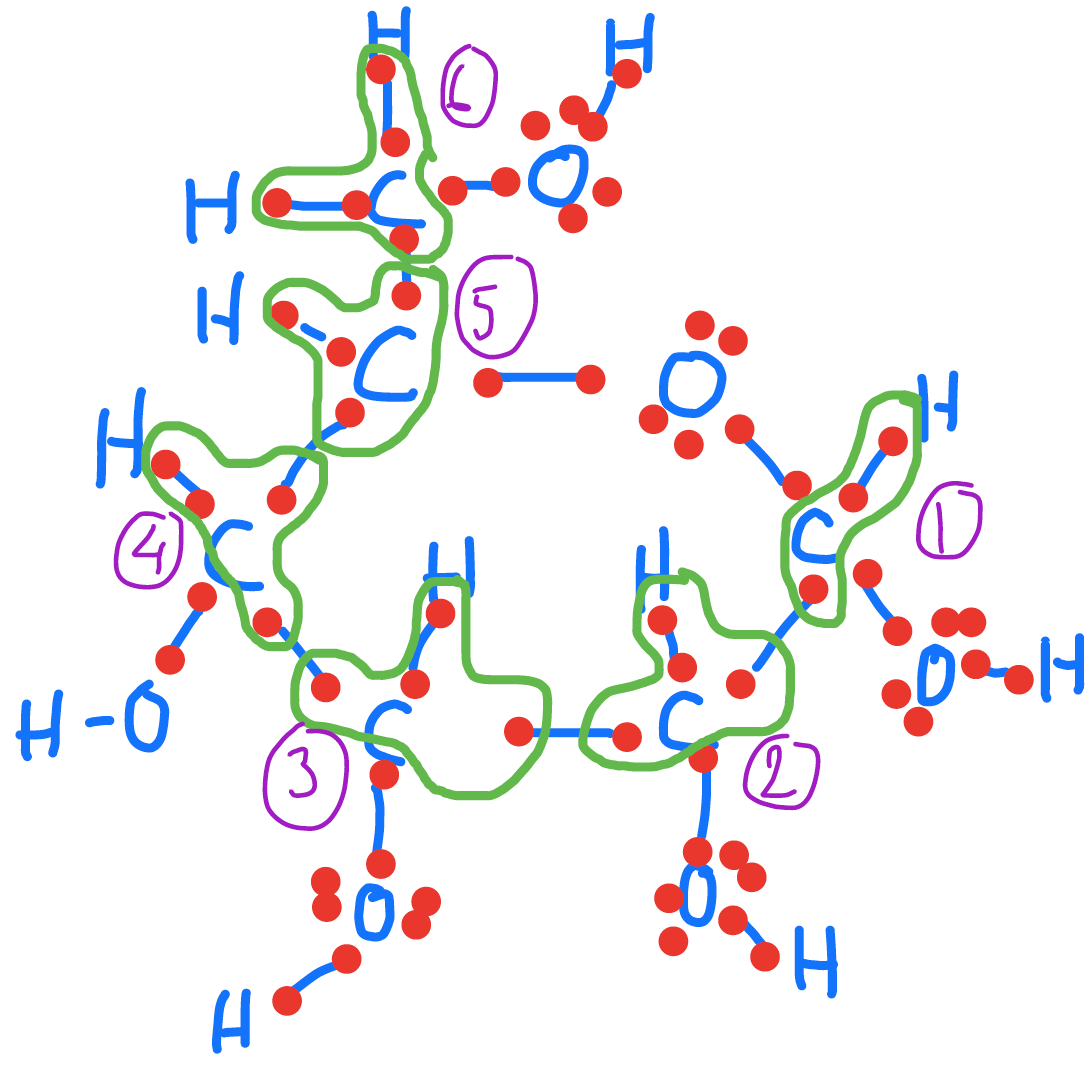
\includegraphics{pictures/ElecAlloc_glucose.png}

N\#2 of nitrous oxide~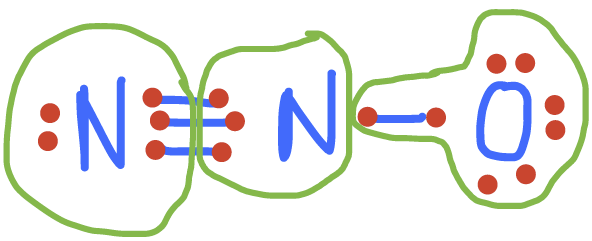
\includegraphics{pictures/ElecAlloc_N2O.png}

4

C\#2 to C\#5 of glucose~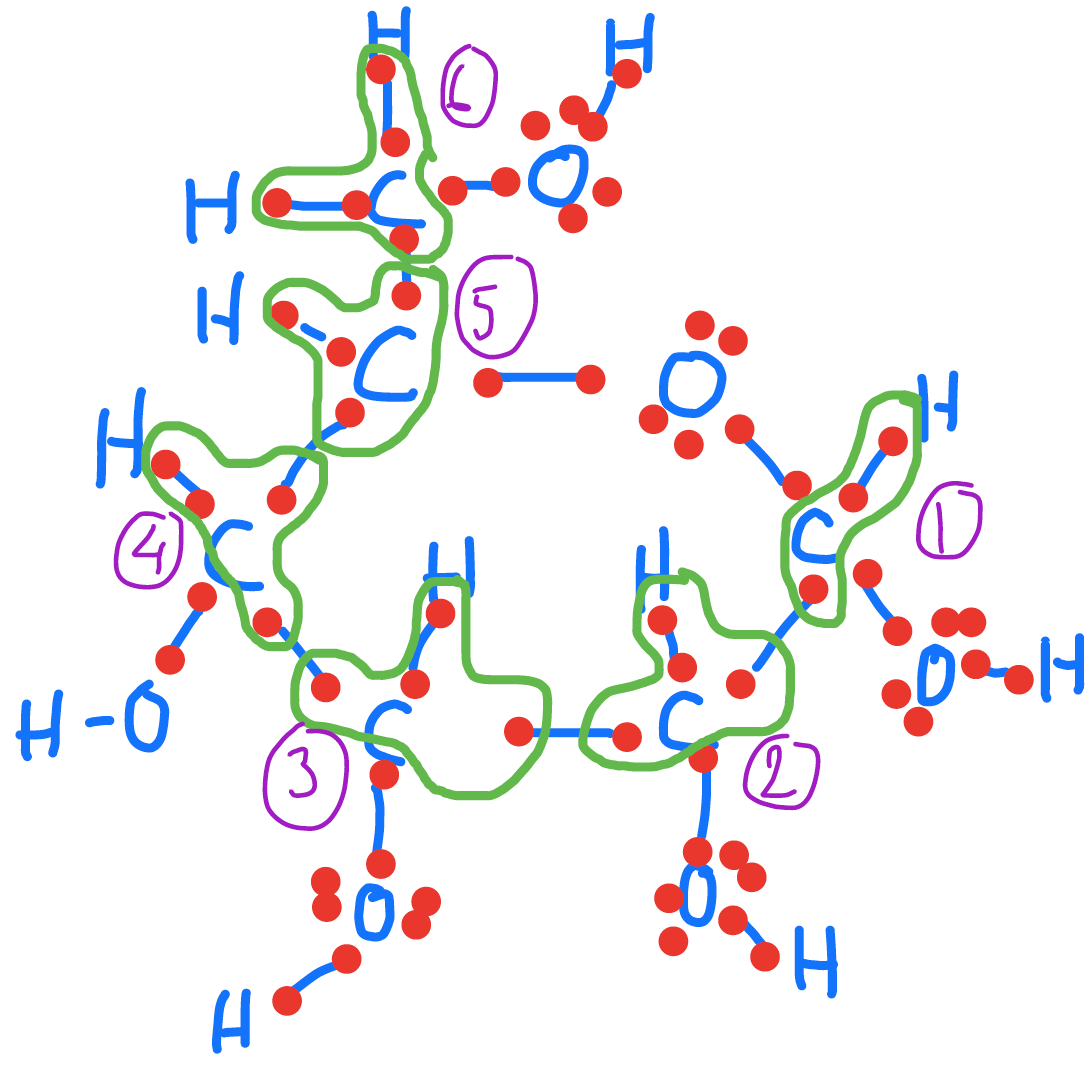
\includegraphics{pictures/ElecAlloc_glucose.png}

5

C\#6 of glucose~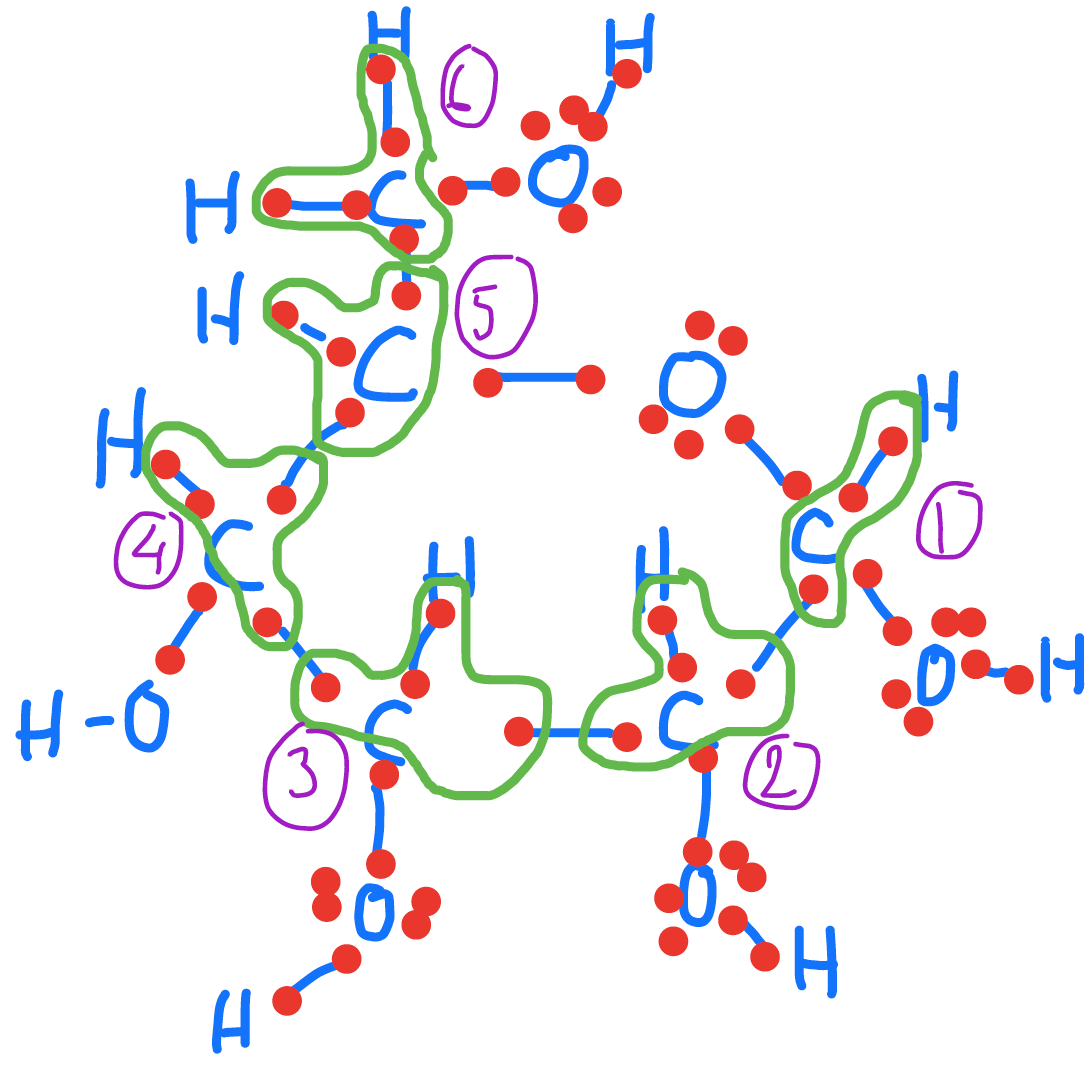
\includegraphics{pictures/ElecAlloc_glucose.png}

dinitrogen~
\includegraphics{pictures/ElecAlloc_N2.png} nitrogen monoxide
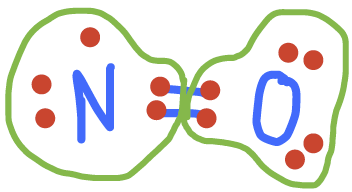
\includegraphics{pictures/ElecAlloc_NO.png} N\#1 of nitrous oxide
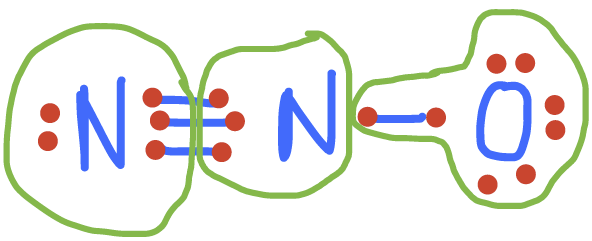
\includegraphics{pictures/ElecAlloc_N2O.png}

6

C of fatty
acid~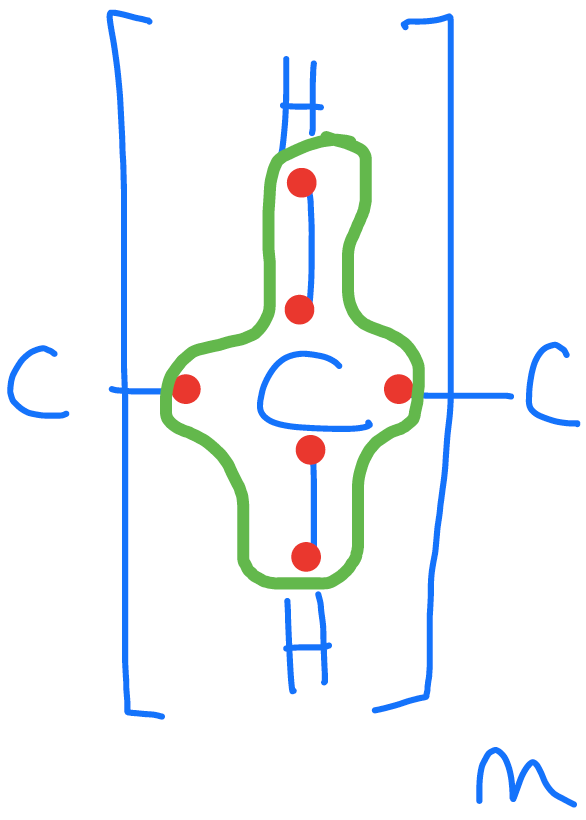
\includegraphics[width=0.70000\textwidth]{pictures/ElecAlloc_fatty_acid.png}

7

pyruvic acid
(C\#3)~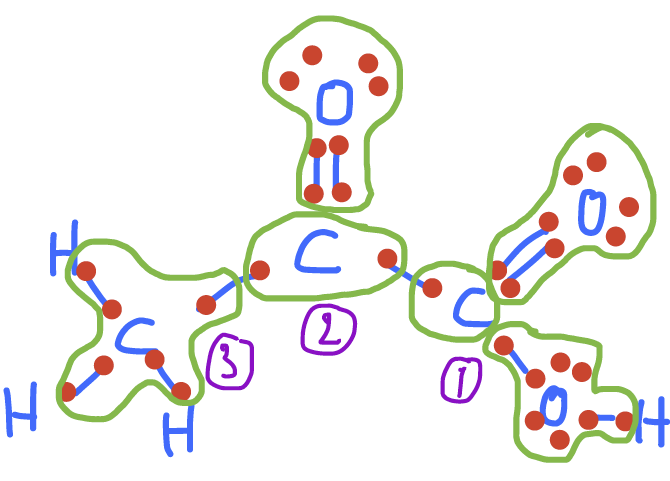
\includegraphics{pictures/ElecAlloc_pyruvic_acid.png}

8

methane~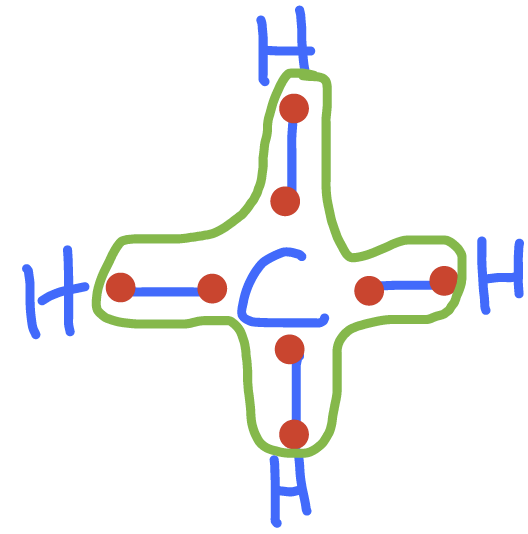
\includegraphics[width=0.70000\textwidth]{pictures/ElecAlloc_CH4.png}

ammonium~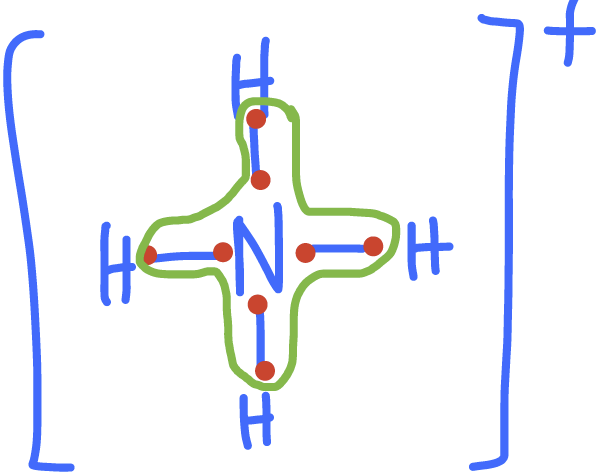
\includegraphics{pictures/ElecAlloc_NH4+.png} ammonia
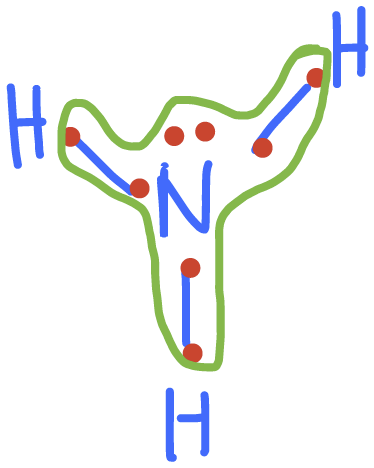
\includegraphics[width=0.70000\textwidth]{pictures/ElecAlloc_NH3.png}
amine groups in amino-acids
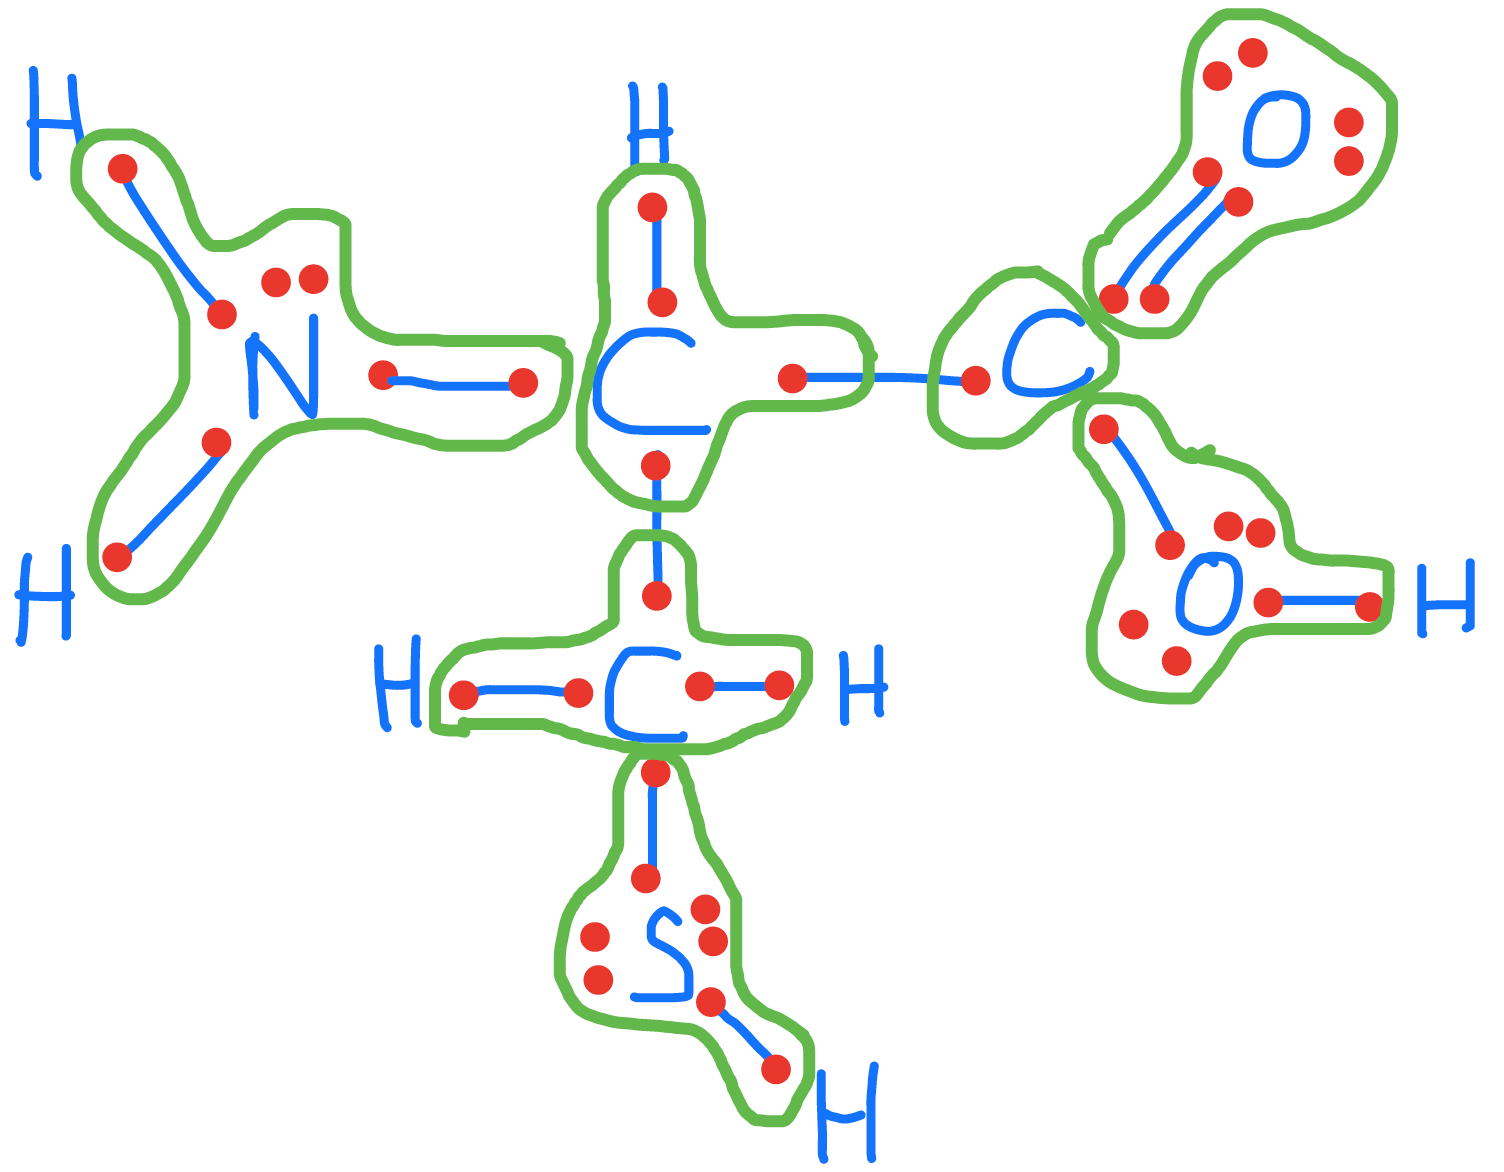
\includegraphics{pictures/ElecAlloc_cysteine.png}

dihydrogen sulfide~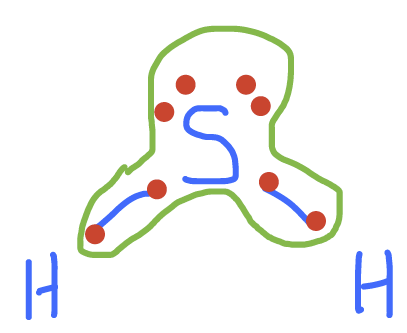
\includegraphics{pictures/ElecAlloc_H2S.png} hydrogen
sulfide 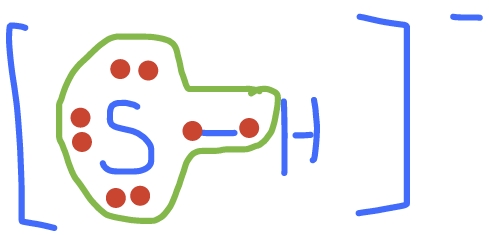
\includegraphics{pictures/ElecAlloc_HS-.png} sulfide
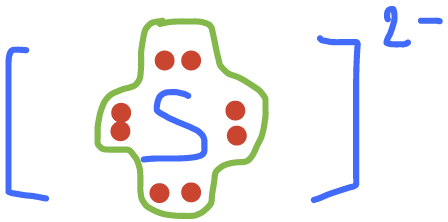
\includegraphics{pictures/ElecAlloc_S2-.png} thiol groups in organic
molecules 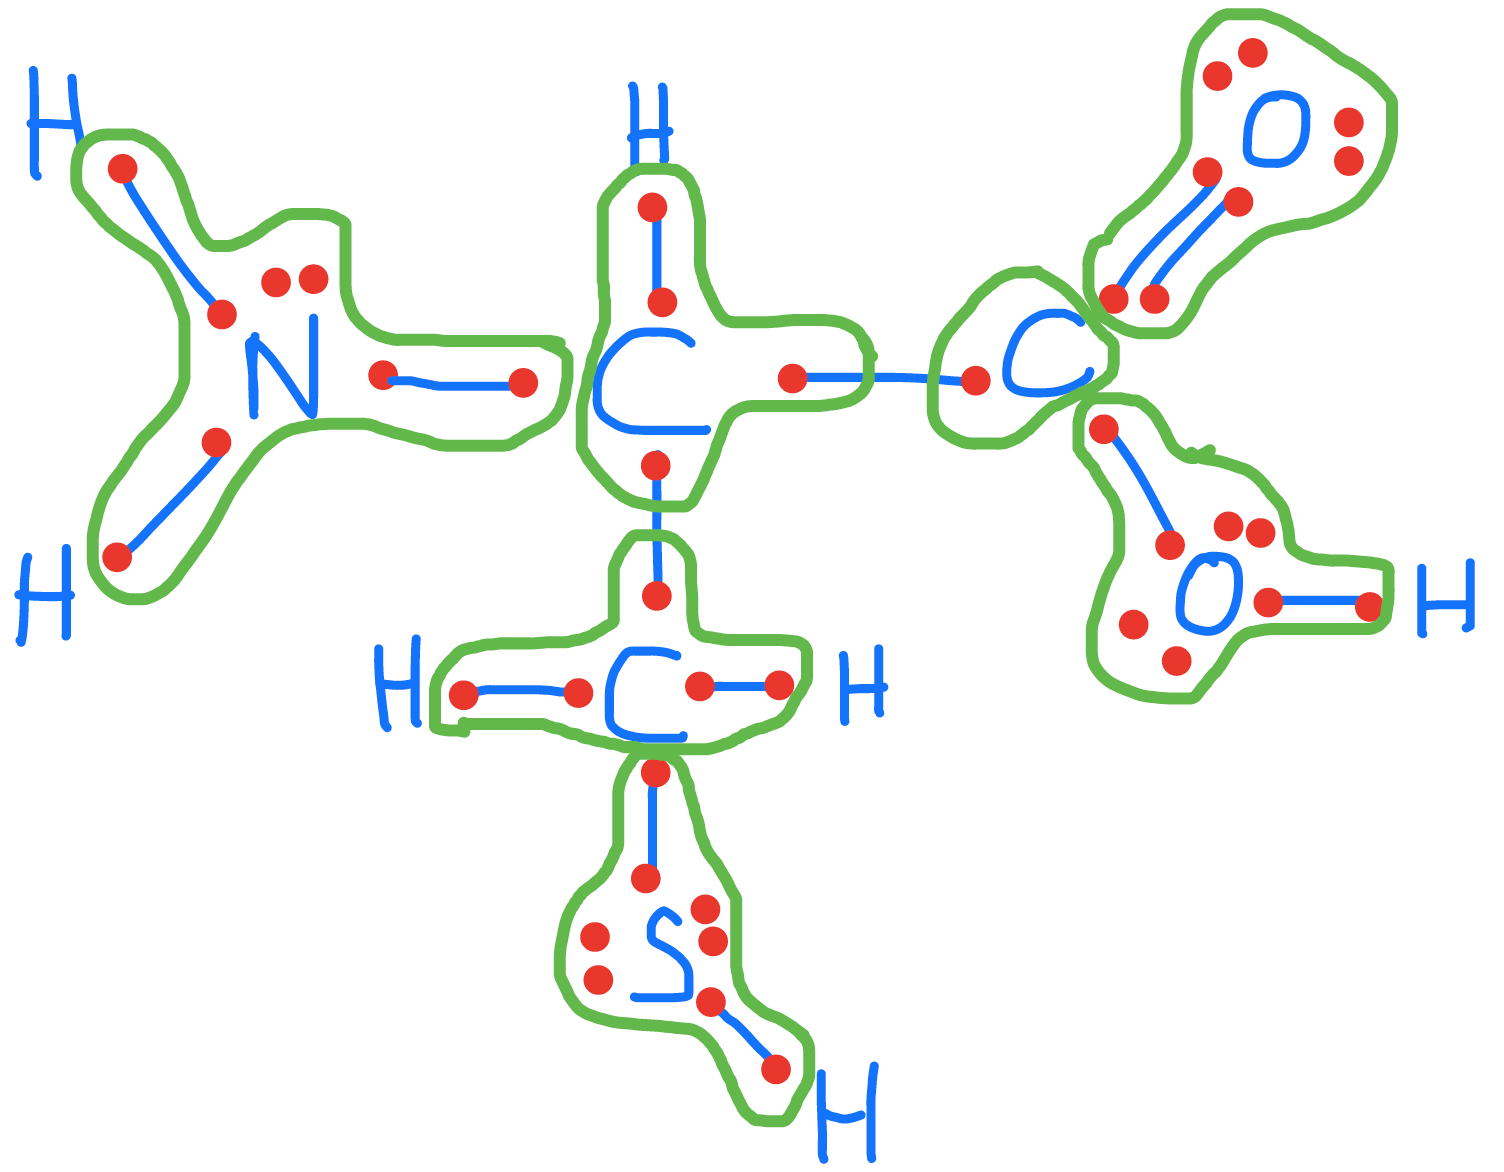
\includegraphics{pictures/ElecAlloc_cysteine.png}

\section{Other important things about code
chunks}\label{other-important-things-about-code-chunks}

Code chunks (but not inline code) can take a lot of \textbf{options}
which modify how they are run, and how they appear in the document.
These options go after the initial \texttt{r} and before the closing
\texttt{\}} that announces the start of a code chunk. One of the most
common options turns off printing out the code, but leaves the results
alone:
\texttt{\textasciigrave{}\textasciigrave{}\textasciigrave{}\{r,\ echo=FALSE\}}
Another runs the code, but includes neither the text of the code nor its
output.
\texttt{\textasciigrave{}\textasciigrave{}\textasciigrave{}\{r,\ include=FALSE\}}
This might seem pointless, but it can be useful for code chunks which do
set-up like loading data files, or initial model estimates, etc.

 Another option prints the code in the document, but does not run it:
\texttt{\textasciigrave{}\textasciigrave{}\textasciigrave{}\{r,\ eval=FALSE\}}
This is useful if you want to talk about the (nicely formatted) code.
Another option on the results of the code is that it generate all
results ``as-is'', which is very nice when your code generates mark-up
text to be rendered by \texttt{Pandoc}.

\texttt{\textasciigrave{}\textasciigrave{}\textasciigrave{}\{r,\ results="asis"\}}
By default, the results of a chunk with have \texttt{\#\#} as a prefix.
You can remove this by putting

\texttt{\textasciigrave{}\textasciigrave{}\textasciigrave{}\{r,\ comment=FALSE\}}

 Sometimes, running of the code will generate warnings and messages.
These can be turned off in the output by using

\texttt{\textasciigrave{}\textasciigrave{}\textasciigrave{}\{r,\ warning=FALSE,\ message\ =\ FALSE\}}

\section{Naming Chunks}\label{naming-chunks}

You can give chunks names immediately after their opening, like
\texttt{\textasciigrave{}\textasciigrave{}\textasciigrave{}\{r,\ clevername\}}.
This name is then used for the images (or other files) that are
generated when the document is rendered.

\section{Adjusting figure sizes and
alignments}\label{adjusting-figure-sizes-and-alignments}

These details are discussed in the accompanying written article on
instantaneous vs.~interval-average flow data.

\subsubsection{\texorpdfstring{``Caching'' Code Chunks (Re-Running Only
When
Changed)}{Caching Code Chunks (Re-Running Only When Changed)}}\label{caching-code-chunks-re-running-only-when-changed}

By default, R Markdown will re-run all of your code every time you
render your document. If some of your code is slow, this can add up to a
lot of time. You can, however, ask R Markdown to keep track of whether a
chunk of code has changed, and only re-run it if it has. This is called
\textbf{caching} the chunk.

\begin{Shaded}
\begin{Highlighting}[]
\KeywordTok{summary}\NormalTok{(cars)}
\end{Highlighting}
\end{Shaded}

\begin{verbatim}
##      speed           dist       
##  Min.   : 4.0   Min.   :  2.00  
##  1st Qu.:12.0   1st Qu.: 26.00  
##  Median :15.0   Median : 36.00  
##  Mean   :15.4   Mean   : 42.98  
##  3rd Qu.:19.0   3rd Qu.: 56.00  
##  Max.   :25.0   Max.   :120.00
\end{verbatim}

One issue is that a chunk of code which hasn't changed itself might call
on results of earlier, modified chunks, and then we \emph{would} want to
re-run the downstream chunks. There are options for manually telling R
Markdown ``this chunk depends on this earlier chunk'', but it's
generally easier to let it take care of that, by setting the
\texttt{autodep=TRUE} option.

\begin{enumerate}
\def\labelenumi{\arabic{enumi}.}
\tightlist
\item
  If you load a package with the \texttt{library()} command, R Markdown
  isn't smart enough to check whether the package has changed (or indeed
  been installed, if you were missing it). So that won't trigger an
  automatic re-running of a cached code chunk.
\item
  To manually force re-running all code chunks, the easiest thing to do
  is to delete the directory R Markdown will create (named something
  like \emph{filename}\texttt{\_cache}) which it uses to store the state
  of all code chunks.
\end{enumerate}

\subsubsection{Setting Defaults for All
Chunks}\label{setting-defaults-for-all-chunks}

You can tell R to set some defaults to apply to all chunks where you
don't specifically over-ride them. Here are the ones I generally use:

This sets some additional options beyond the ones I've discussed, like
not re-running a chunk if only the comments have changed
(\texttt{cache.comments\ =\ FALSE}), and leaving out messages and
warnings. (I'd only recommend suppressing warnings once you're sure your
code is in good shape.) I would typically give this set-up chunk itself
the option \texttt{include=FALSE}.

You can over-ride these defaults by setting options for individual
chunks.

\subsubsection{More Chunk options}\label{more-chunk-options}

See {[}\url{http://yihui.name/knitr/options/}{]} for a complete listing
of possible chunk options.

\chapter{Referencing and Cited
References}\label{referencing-and-cited-references}

\section{Autoreferencing}\label{autoreferencing}

The beauty of the system is that the referencing is all automatised.

\begin{itemize}
\tightlist
\item
  So to reference an equation use
  \texttt{\textbackslash{}@ref(eq:HnApoly)} to obtain equation
  \eqref{eq:HnApoly}
\item
  So to reference a figure
  use\texttt{\textbackslash{}@ref(fig:molarfracPO4)} to obtain figure
  \ref{fig:molarfracPO4}
\item
  So to reference an table
  use\texttt{\textbackslash{}@ref(tab:ElecAllocTab)} to obtain table
  \ref{tab:ElecAllocTab}
\end{itemize}

\section{Cited references}\label{cited-references}

I have created and maintained for over 15 years a database written in
Microsoft Access of around 2000 articles, most of them photocopied and
typed in the database by hand during and after my Ph.D. (yes, I should
have a medal!\ldots{}) but I have to admit that this system is past its
time\ldots{} I have now switched to Paperpile. There are many other
referencing software out there now
(\href{https://en.wikipedia.org/wiki/Comparison_of_reference_management_software}{a
list and comparison can be found here}). The beauty of them is that they
will all export in recognized formats and this is what we care about
here. So no more copy/paste of references from some pdf. We are going
into \emph{reproducible research}. This means that all the articles you
want to work with will be entered in the reference database of your
choice. Make sure you start one ASAP!

In the YAML header, you can now see
\texttt{bibliography:\ {[}book.bib,\ packages.bib{]}}. This means that
there are files named \texttt{book.bib} and \texttt{packages.bib} that
are located in the same directory as the all the .Rmd files, which when
we `knit', \href{https://pandoc.org/MANUAL.html}{Pandoc} will look for.
You can access these \texttt{.bib} file in the GitHub directory. There
is actually a possibility to add within the \texttt{.Rmd} document
itself, the text needed for Pandoc to read the references, but unless
you only have very few references, this can become very messy quickly.
See the
\href{http://rmarkdown.rstudio.com/authoring_bibliographies_and_citations.html\#bibliographies}{RStudio
Bibliographies documentation} for more details.

In short, in this file, there is a list of articles which information is
coded according to the format chosen. By the way, a lot of the details
for the bibliography are available on the
\href{http://rmarkdown.rstudio.com/authoring_bibliographies_and_citations.html\#bibliographies}{RStudio
Bibliographies documentation}. R Markdown will recognize up to 10
different formats. The one Paperpile exports is \texttt{.bibtex}, so
this is the one I have usually add in the YAML header. The filename
extension will determine the \emph{rendering} process, so make sure you
have the right extension as well.

So, in the \texttt{.bib} file I have, the first article appears as

\begin{verbatim}
@ARTICLE{Kuhne2009-tn,
  title   = "Improving the Traditional Information Management in Natural
  Sciences",
  author  = "K{\"u}hne, Martin and Liehr, Andreas W",
  journal = "Data Sci. J.",
  volume  =  8,
  pages   = "18--26",
  year    =  2009,
  issn    = "1683-1470, 0308-9541",
  doi     = "10.2481/dsj.8.18"
}
\end{verbatim}

here is another reference \citep{Maxwell2018-ht} or this website
\citep{Wikipedia_contributors2018-ia}

The first item after ``ARTICLE\{'' is the unique identifier for the
article. The identifier of this article is \texttt{Kuhne2009-tn}. When
one wants to cite this article, one will say something like
``reproducible research has been suggested to become the norm
\citep{Kuhne2009-tn}''. And you would code like

\begin{verbatim}
"reproducible research has been suggested to become the norm [@Kuhne2009-tn]"
\end{verbatim}

If you want to say that ``Kühne et al. \citeyearpar{Kuhne2009-tn} have
shown that etc.'', you would add a ``dash'' just before the ``@'' and
code it as such:

\begin{verbatim}
Kühne et al. [-@Kuhne2009-tn] have shown that etc."
\end{verbatim}

If you want to cite several references, you would add a semicolon
between the two such as in:

\begin{verbatim}
"reproducible research has been suggested to become the norm [@Kuhne2009-tn; @Buckheit1995-ls]"
\end{verbatim}

Notice that among all the fields from the example above, there are
\texttt{doi} and \texttt{issn}. \texttt{doi} stands for ``Digital Object
Identifier''. \texttt{issn} stands for International Standard Serial
Number (ISSN), which is an eight-digit serial number used to uniquely
identify a serial publication. The \texttt{doi} value in this example is
\texttt{10.2481/dsj.8.18}, which is unique in the world. These
\texttt{doi} are applied to articles but not only. They are also applied
to data. Eventually, all data that will be used in an article will have
to have its own \texttt{doi} and all the codes that are used to analyze
the data will refer to this unique \texttt{doi}. This is not quite
implemented yet (in 2017), but will likely be by 2022. \texttt{doi} or
\texttt{url} (not added here; stands for Uniform Resource Locator. Quite
a mouthful, really, for what it is: a web address) are not necessarily
exported from your reference software by default. Make sure you add this
possibility, as \texttt{doi} is almost routinely added in the reference
list in most journals.

The reference list of the citations will appear right after you place

\begin{verbatim}
# References
\end{verbatim}

at the bottom of your Rmd docucment, if it a single Rmd document, or as
a separate chapter for a book. When rendering your document, the list
will appear automatically afterwards, and if you have in text notes,
these will appear underneath.

\subsection{Link to citations}\label{link-to-citations}

In a single Rmd document (not a book) One very nice feature is to create
hyperlinks from the in-text citations to the citations in the reference
section. For this, just add \texttt{link-citations:\ true} in the YAML
header.

\subsection{CSL and styling of
citations}\label{csl-and-styling-of-citations}

CSL stands for Citation Style Language. The CSL line command is an
option for the citation styles to be used in your document. You can
comment it out by adding a ``\#'' in front of it and the default .CSL
file will apply without you noticing it. Each journal has its own way of
handling how an article/reference should be cited in the text, and in
the reference section, and there are hundreds of different styles out
there\ldots{} You can read lots of details on this
\href{http://docs.citationstyles.org/en/stable/primer.html}{CSL primer}
about how all this works.

While I was writing this tutorial, I did not specify at first the
citation style. And I kept getting, using the same example as before,
``(Kühne and Liehr 2009)'', although I wanted ``(Kühne and Liehr,
2009)'', i.e., with a comma between the authors and the date, because
this is the way I always did it and I think it is a lot better this way.
Then I started thinking about the journals for which the inline
citations are numbers, sometimes in brackets, sometimes without
brackets\ldots{} what a nightmare\ldots{}! Actually it is extremely
simple: all this is done automatically when you specify the CSL
corresponding to the journal style following which you wish to write.

For this, you can pick at
\url{https://github.com/citation-style-language/styles} the *.CSL file
you are looking for (actually there are too many of them and they are
not all displayed). The fastest way is to Google `` CSL'', and you will
land on the CSL file you are looking for. I recommend that you click on
the \texttt{raw} icon on GitHub, and copy all the file in a text editor.
Warning! You need to make sure that your text editor does not add any
weird formatting or add an extension at the end of the file. I had that
problem and I could not see the extension on my computer, although I had
the option to display so. Save the file in the same directory as your
.Rmd.

So, to go back with my struggling to style the inline citation and the
``missing comma'', it turns out that the default CSL file uses a
``\href{http://rmarkdown.rstudio.com/authoring_bibliographies_and_citations.html\#citation_styles}{Chicago
author-date format}'' (I am not sure what this means exactly), which in
text styling is ``(author date)'', without the comma\ldots{}! If you use
``journal-of-hydrology.CSL'', you will see that all of a sudden after
you \texttt{knit}, the commas just appeared\ldots{}! Eureka! If you use
``nature.CSL'' (because we all want to be ready when we publish in
Nature!), you will see that there are no more in-line citations, just
numbers in superscript, hyphenated when needed, and the references are
all in order, with the journal names in italics, the journal volume in
bold, the year in parenthesis at the end, etc.! Is not that wonderful?
Without your doing anything, other than adding the citation properly in
the text following the guidelines above.

You can, if you want and have a lot of time to waste, take existing CSL
files and modify them to have your own custom citation style. Make sure
you take an ``independent'' CSL file and modify it. Most of them are
dependent upon a ``source'' or independent one, and the code in the CSL
file is just saying how the dependent file should slightly alter the
independent one. Good instructions on how to do this can be found on the
excellent
\href{http://docs.citationstyles.org/en/stable/primer.html}{CSL primer}.

\chapter{Final words}\label{final-words}

Now, it is your time to play!!

\bibliography{book.bib,packages.bib}


\end{document}
